\section{Implementation Details}\label{sec:impl}

\subsection{GetInTUM Android Application}\label{sec:android}


\subsubsection{Android architecture}
The Android app architecture consists of two activities. The $MainActivity$ is responsible for the registration process with the backend and the $UnlockProgressActivity$ provides a UI that shows the status of the NFC-communication after the registration process is complete. To provide a standard Android look and feel, the $MainActivity$ is using a ViewPager to guide the user through the different registration steps. Therefore, the three registration steps (send ID, activate token, finish registration) are represented as fragments.

To initialize all fragments at once (normally, the $onCreate()$ only gets called by adjacent pages of the current page), the $setOffscreenPageLimit$ must be set to the number of pages, three in this case.

When sliding to a specific fragment, its content should be updated. To provide this functionality, a $setOnPageChangeListener$ must be added to the ViewPager to detect a page selection. There, the $OnPageSelected()$ method can be overwritten to call the $onRefresh()$ method of the page. As a result, every fragment implements an $OnRefreshListener$ interface that contains this $onRefresh()$ method.

To keep track of the registration progress, the $SharedPreference$ model of Android is used internally. It makes it very simple to access the app data from different activities and fragments while the content stays consistent.

A $Backend$ class is responsible for the backend communication over HTTPS/TLS. Since the certificate of the backend server is self signed, the certificate must be shipped with the app in the assets folder as a $*.crt$ file. The constructor of the backend then needs to manually create a $CertificateFactory$ as well as a $KeyStore$ containing the one certificate to create the final SSL context.
For certificate pinning, it is a good advice to only store valid certificates of the backend infrastructure in the corresponding $*.crt$ file.

Android forbids network operations in the UI-Thread by design. That is why every backend request is embedded in an $AsyncTask$ showing a progress circle. It can also be aborted by the user if the backend is not reachable.

\subsubsection{NFC Background Service}
As described in more detail in the subsequent section \ref{sec:comm}, the Raspberry Pi acts as a NFC reader and the matching Android device behaves like a NFC card.
For NFC Host-based Card Emulation (\textit{HCE}), Android's HCE service is used to route incoming NFC requests to the \app application. In our implementation, this is \texttt{CardEmulationService}.
This is also the place where the initial connection with the terminal is negotiated and where message fragmentation comes in.
Incoming data chunks are aggregated in a \texttt{ByteArrayOutputStream} with the function \texttt{pushDataChunk}.
Outgoing data chunks are retrieved and segmented from \texttt{ByteArrayInputStream} by the function \texttt{receiveDataChunk}.

%
Due to the fact that the HCE service is based on a common Android service, it is restricted to the same UI thread as the main application.
There are two problems that arise from this situation:
%
\begin{itemize}
	\item Doing complex NFC communication on the main thread might reduce the responsiveness of the visible UI.
	\item NFC readers require immediate feedback from a card. In our case, the emulated card must always response although still having to finish some cryptography, for instance.
\end{itemize}
%
A single threaded model cannot provide a proper solution to those circumstances.

%
\begin{figure}[h]
    \centering
    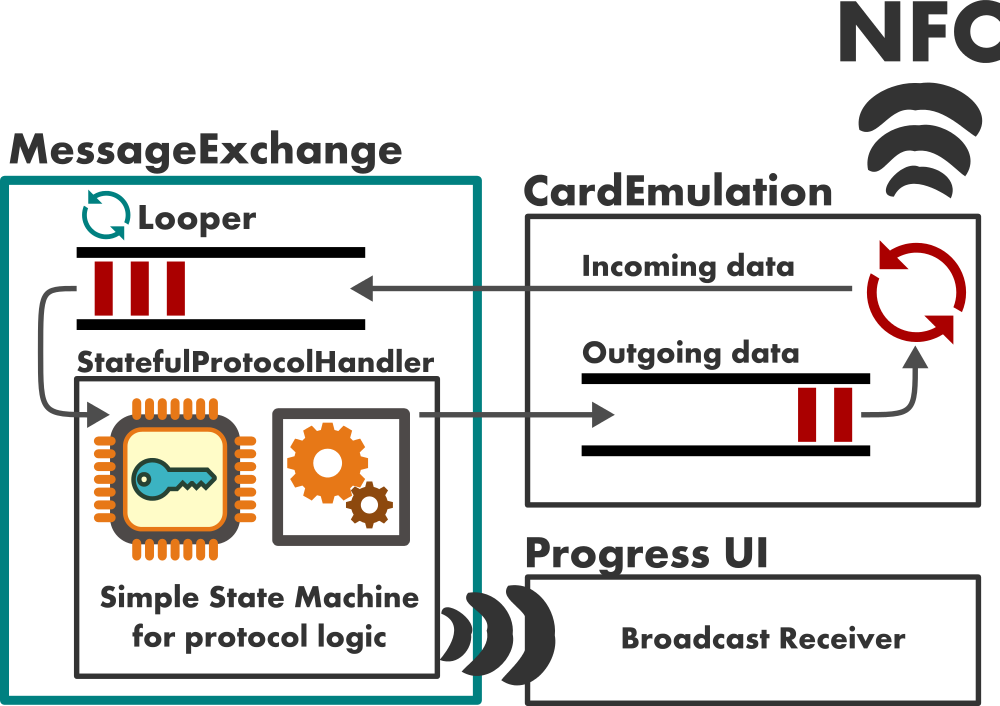
\includegraphics[width=.6\linewidth]{android_nfc_architecture}
    \caption{Android NFC architecture.}
    \label{fig:android:nfc_arch}
\end{figure}
%
Therefore, Android offers the looper framework that allows to process tasks in a separate thread and provides a message passing infrastructure to communicate with the looper thread in a safe way.
For the application, this framework is embedded within a second service \texttt{MessageExchangeService} which is started on demand if there is a connection to a known terminal.
When the \texttt{CardEmulationService} finishes data packets, 
%Involving NFC Host-based Card Emulation,  